\section{Architecture}
\label{architecture}
Our ViT Architecture in Figure \ref{fig:ViTArchi} follows a three-stage process to process an input image:
\begin{itemize}
    \item Patch Selection: The input image is divided into a grid of fixed-size non-overlapping patches, typically 16x16 pixels in size. For each patch is calculated a score based on an heuristic (contrast/variance/entropy). The calculated values are interpreted as a probability distribution and a $k$ sample of patches is selected and passed to next step. The number of patches is determined by the size of the input image and the patch size.
    \item Patch Embeddings:  Each patch is then linearly projected to a low-dimensional space to obtain a patch embedding vector. The patch embeddings are arranged in a sequence to form the input to the transformer encoder. 
    \item Transformer Encoder: The patch embeddings are fed into a modified transformer encoder, which consists of multiple identical layers of self-attention and feed-forward layers. The self-attention mechanism allows the model to attend to different parts of the image and model the spatial relationships between patches. The feed-forward layers process the information from the previous layers and output a sequence of feature vectors.
\end{itemize}


    \begin{figure}[htp]
        \centering
        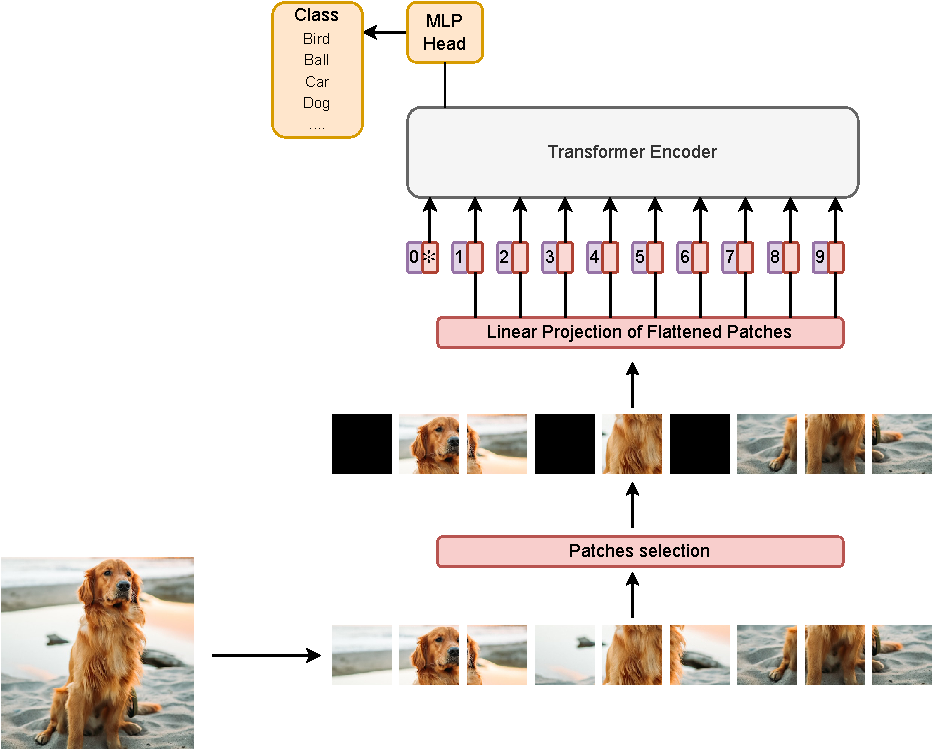
\includegraphics[height=7cm]{images/Vision Transformer Diagram.drawio.pdf}
        \caption{Our ViT Architecture}
        \label{fig:ViTArchi}
    \end{figure}


In this particular implementation, figure \ref{fig:TransformereNCODER}, of the Transformer Encoder block, the Multi-Head Attention layer has been modified to be probabilistic in nature. Specifically, the attention weights computed by the layer are used as mixture weights and the values associated with each key are used as the component of the PDFs.

This modification allows for a more flexible and expressive representation of the attention mechanism. By using a probabilistic approach, the model can capture a wider range of dependencies between different positions in the sequence.
    \begin{figure}[htp]
        \centering
        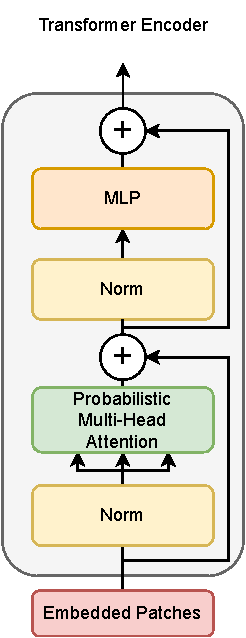
\includegraphics[height=7cm]{images/Transformer Encoder.drawio.pdf}
        \caption{Modified Transformer Encoder Block}
        \label{fig:TransformereNCODER}
    \end{figure}
